
\hypertarget{sec:hockling}{%
\subsection{Flexible Rod Buckling Under Torque}\label{sec:hockling}}
\begin{figure}[h]
\centering
\begin{subfigure}[b]{0.49\textwidth}
\centering
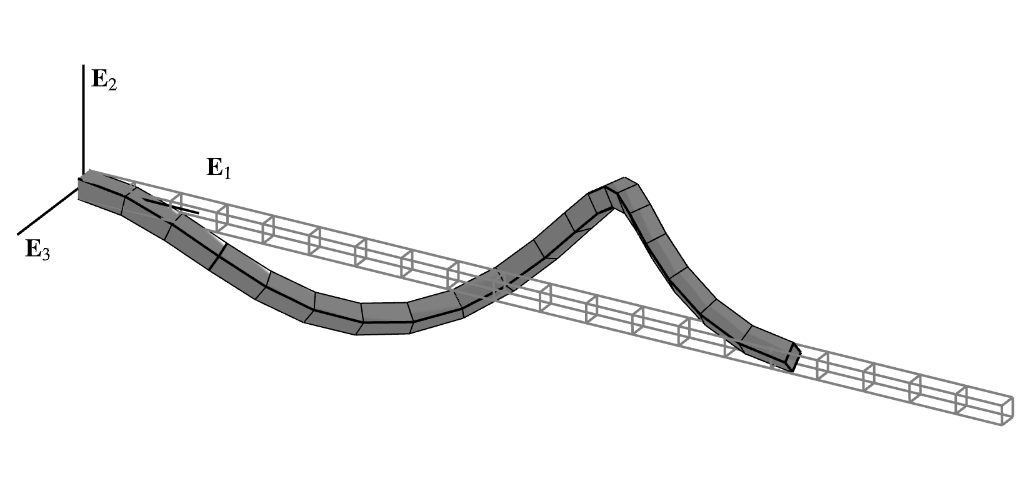
\includegraphics[width=0.95\textwidth,keepaspectratio]{Figures/Figure_4a}
\caption{\(\tau = 20\)}
\end{subfigure}
\begin{subfigure}[b]{0.49\textwidth}
\centering
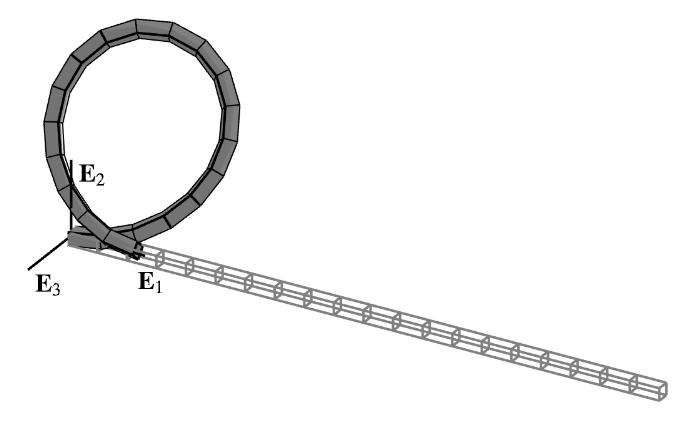
\includegraphics[width=0.8\textwidth,keepaspectratio]{Figures/Figure_4b}
\caption{\(\tau = 60\)}
\end{subfigure}
\caption{Deformed shapes of hockling rod at various pseudo-time steps \(\tau\).}
\label{fig:hockling}
\end{figure}
The hockling problem in Figure \ref{fig:hockling} is a particularly complex problem that arises from practical considerations for the design of propeller shafts in large ships \citep{rosenthal1976application,oreilly2017modeling}.
The problem is posed as a propped cantilever with
a torque \(T\,\mathbf{E}_1\) applied at its end \(\xi = L\). 
The rod is fixed at the origin and is free
to translate along the \(\mathbf{E}_1\) direction at its end. 
% which is applied by fixing all degrees of freedom at \(\xi=0\), and \(2, 3, 5,\) and \(6\) at \(\xi = L\).
This problem was investigated analytically by
\cite{greenhill1883strength,ziegler1977principles} who found an \emph{approximate} minimum buckling torque \(T_{\mathrm{cr}}\) given by:
\[
T_{\mathrm{cr}} = \lambda_{\text{cr}} \frac{2 EI}{L}
\qquad\text{ where }\qquad
\lambda_{\text{cr}}  = \min  \left\{\lambda  \mid \tan \lambda - \lambda = 0\right\} \approx \pm 4.493409
\]
\citet{ziegler1977principles} reports the value \(\lambda_{\text{cr}} \approx \pm 4.494\), which is commonly used in the literature. 
Because the loaded end is constrained to rotate about a fixed
axis, all rotation parameterizations coincide at this node so that, in all cases, the moment can be applied by simple scaling of a reference vector.

The following parameters are commonly adopted for the problem \citep{nour-omid1991finite,saleeb1992effective}:
\[
\begin{array}{lcr}
    L &=&   240 \\ %   ,& A  &= 10 \\
    E &=& 71240 \\ %   ,& I  &= 0.0833 \\
    G &=& 27190 \\ %   ,& J  &= 2.16 \\
\end{array}
\qquad\qquad
\begin{array}{lcr}
    A &=& 10\hphantom{.0833}  \\
    I &=& 0.0833 \\
    J &=& 2.16\hphantom{33}   \\
\end{array}
\]
To induce bifurcation, the undeformed
centerline \(\boldsymbol{x}_0(\xi)\) is slightly rotated off the axis of the roller reaction:
%
\begin{equation*}
\boldsymbol{x}_0(\xi) = \xi \operatorname{Exp}\begin{pmatrix}
  0 \\ 10^{-3} \\ 0
\end{pmatrix} \mathbf{E}_1 .
\end{equation*}
%
The simulation uses a discretization of 20 elements for the rod, and the torque is applied in 65 increments with iterative and incremental load factor control. The analysis uses the \texttt{SFIN} isometry with both \texttt{None} and \texttt{Incr} interpolation and parameterization variants.
Figure~\ref{fig:hockle-plot} shows the relation between load factor \(\lambda\) and end rotation \(\vartheta = \|\operatorname{Log}\boldsymbol{\Lambda}(L)\|\).
%
This figure shows that the buckling load of the simulation is slightly higher than the value derived by \cite{ziegler1977principles}, but 
is consistent with findings for geometrically exact elements in the literature \citep{nour-omid1991finite,ibrahimbegović1996role,saleeb1992effective,santos2011hybridmixed}.

\begin{figure}[!h]
    \centering
    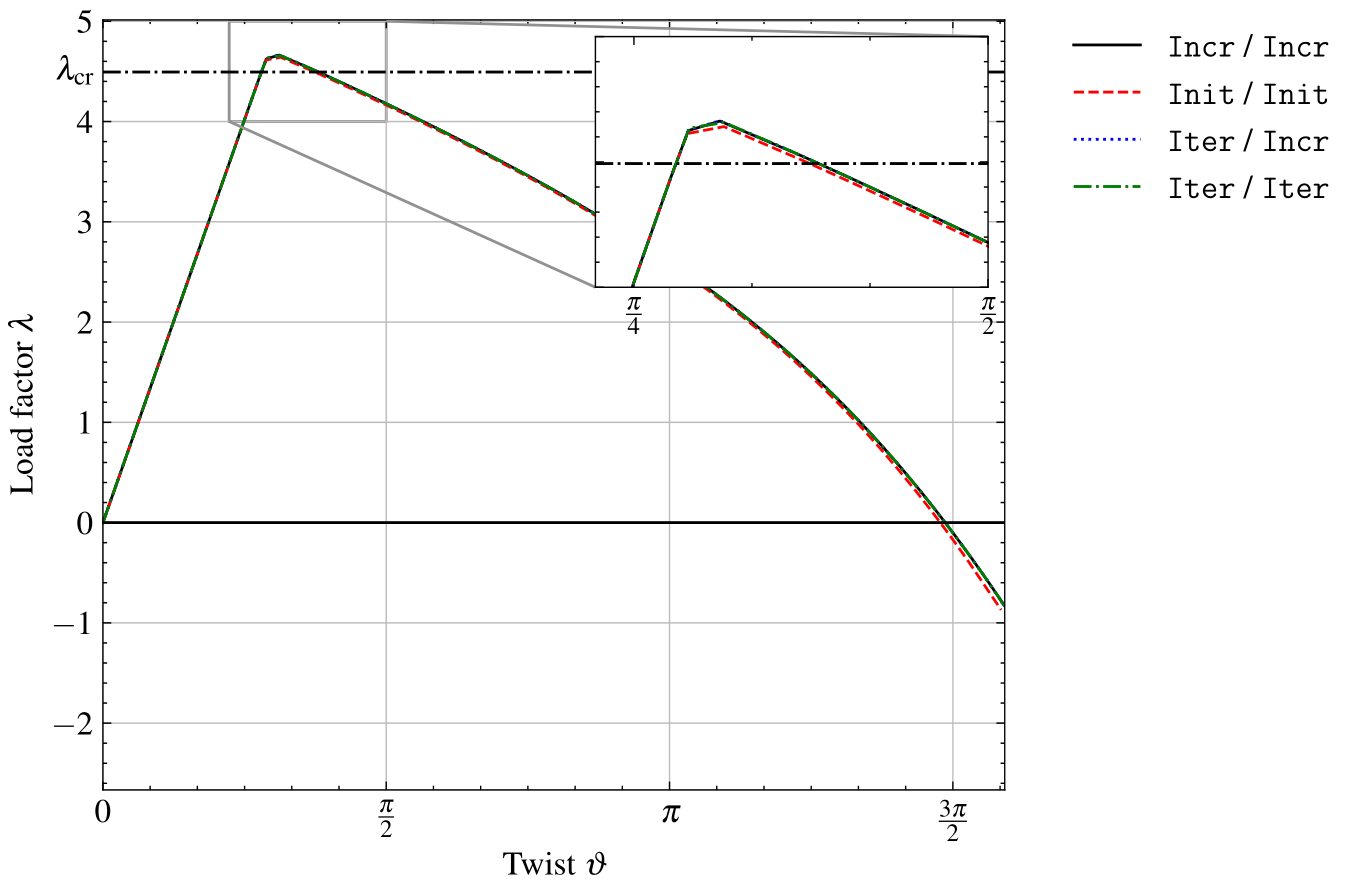
\includegraphics[width=0.7\textwidth]{Figures/Figure_5}
    \caption{Relation between load factor \(\lambda\) and end rotation angle \(\vartheta\) for the hockling problem with the \texttt{SFIN} isometry and different interpolation/parameterization pairs.}
    \label{fig:hockle-plot}
\end{figure}
